\documentclass[a4paper,11pt]{article}
%\usepackage[T1]{fontenc}

%\setlength{\textwidth}{20cm}
%\setlength{\marginparwidth}{0cm}
%\setlength{\voffset}{0cm}
\usepackage[utf8]{inputenc}
\usepackage[francais]{babel}
\usepackage{amsmath}
\usepackage{graphicx}
\usepackage{subfig}
\usepackage{hyperref}
\usepackage{karnaugh-map}
%\special{papersize=210mm,297mm}

\newcommand{\op}{
  \mathop{
    \vphantom{\bigoplus}
    \mathchoice
      {\vcenter{\hbox{\resizebox{\widthof{$\displaystyle\bigoplus$}}{!}{$\boxplus$}}}}
      {\vcenter{\hbox{\resizebox{\widthof{$\bigoplus$}}{!}{$\boxplus$}}}}
      {\vcenter{\hbox{\resizebox{\widthof{$\scriptstyle\oplus$}}{!}{$\boxplus$}}}}
      {\vcenter{\hbox{\resizebox{\widthof{$\scriptscriptstyle\oplus$}}{!}{$\boxplus$}}}}
  }\displaylimits
}

\title{{\Huge Electronique numérique}\\Automates (1)}
\date{}

\begin{document}
\maketitle
{\it Tous les exercices ne seront pas forcément résolus en TE.}\\

Ce TD aborde plusieurs points relatifs aux {\it automates}, aussi appelés {\it machines d'états finis}
\footnote{Ce nom quelque peu étrange signifie que le {\it nombre} d'états est {\it fini}. Il existe également
des automates dont le nombre d'états est infini...}{\it finite state machines} (FSM).
\begin{itemize}
  \item Diagrammes états transitions : machines de Mealy et de Moore.
  \item Causalité des machines d'états finis.
  \item Conception d'un automate matériel à partir d'un diagramme  états-transitions.
\end{itemize}


\section{Diagramme états-transitions. Moore et Mealy}
On rappelle que le diagramme à bulle (ou ``state transition diagram'' ou diagramme ``états-transistions'') est une représentation graphique pratique des automates.
Elle consiste à décrire l'enchaînement des transitions d'un état à l'autre par une flèche,
les états étant représentés par des cercles ou ``bulles''.

On distingue deux grands types de FSM (voir figure \ref{fig:example}) \footnote{Attention !
Les deux automates représentés l'un à côté de l'autre ne sont pas équivalents en terme de fonctionnement.
Il existe des algorithmes pour transformer Mealy en Moore (et réciproquement), de manière à obtenir des
comportements identiques.... Voir par exemple \url{https://fr.wikipedia.org/wiki/Machine_de_Mealy})}. Dans le cas des automates de Moore, les sorties ne dépendent que des états, alors que dans le cas des automates de Mealy,
les sorties dépendent à la fois des états et des entrées. Sur les transitions, on ajoute les {\it conditions} booléennes $c_i(s)$ qui autorisent à passer d'un état à un autre, ainsi
que d'éventuelles sorties (généralement après une ou deux barres verticales) dans le cas des automates de Mealy. Lorsqu'on a affaire à un automate de Moore, les sorties sont annotées en
conséquence dans les bulles (ou juste à côté !).\\

\begin{figure}[!h]
    \centering
    \subfloat[label 1]{{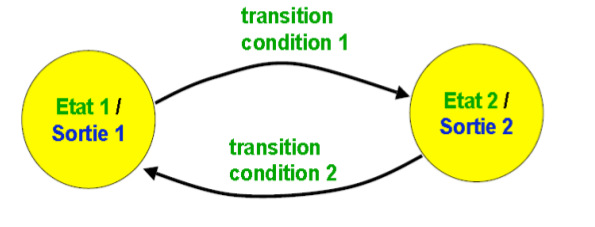
\includegraphics[width=5cm]{./figures/moore.png} }}%
    \qquad
    \subfloat[label 2]{{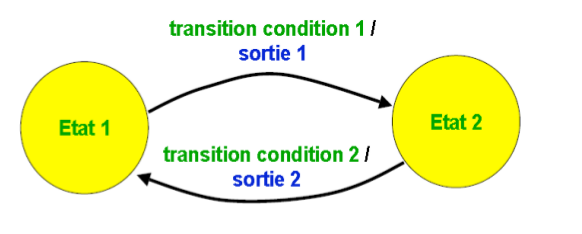
\includegraphics[width=5cm]{./figures/mealy.png} }}%
    \caption{FSM de Moore et Mealy}%
    \label{fig:example}%
\end{figure}


\section{Causalité d'une FSM}
Pour que qu'une FSM  soit considérée comme {\it causale}, correcte ou {\it consistante}, elle doit vérifier les deux propriétés suivantes :
\begin{itemize}
\item \textbf{Réactivité} (exhausitivité): il doit exister une condition vraie sur au moins une des transitions sortant d'un état.
$$\forall s \in S : \sum_i c_i(s)=1$$
\item \textbf{Déterminisme} (exclusivité): deux conditions sur les transitions sortant d'un état ne peuvent être vraies en même temps.
$$\forall s \in S, \forall (i,j) \text{ avec } i \neq j, c_i(s).c_j(s)=0$$
\end{itemize}

Une autre manière de résumer ces deux propriété est qu'il existe -- à tout instant discret -- {\it un, et un seul, état suivant}.

Notons qu'un état peut avoir comme état suivant lui-même : dans ce cas, le système décrit ne change pas d'état.\\

%%$$\forall s \in S : \sum_i c_i(s)=1$$
%%$$\forall s \in S , c_1(s) \oplus c_2(s) ... \oplus c_n(S) = 1$$

%% \begin{figure}[!h]
%% \begin{center}
%% \includegraphics[scale=0.2]{./d-ff-infos.jpg}
%% \end{center}
%% \end{figure}
Observez la figure \ref{fig2}.
\begin{itemize}
\item Vérifier la consistance de la machine d'état suivante.
\item Est-ce un automate de Moore ou de Mealy ?
\end{itemize}

\boxed{corrections}
Il y a plusieurs manières de procéder. Par exemple, on calcule les formules :

\begin{itemize}
\item exhausitivité :

\begin{itemize}
\item Pour S0 : $\overline{e_1}+e_1=...=1$
\item Pour S1 : $\overline{e_2}+\overline{e_1}.e_2+e_1.e_2=...=1$
\item Pour S2 : $1=\dots=1$
\end{itemize}

\item exclusivité :
\begin{itemize}
\item Pour S0 : $\overline{e_1}.e_1=...=0$
\item Pour S1 : $\overline{e_2}.\overline{e_1}.e_2+\overline{e_2}.e_1.e_2+\overline{e_1}.e_2.e_1.e_2=0+0+0=0$
\item Pour S2 : une seule transition. Il n'y a pas de problème d'exclusivité.
\end{itemize}

\end{itemize}

\begin{figure}[!h]
\begin{center}
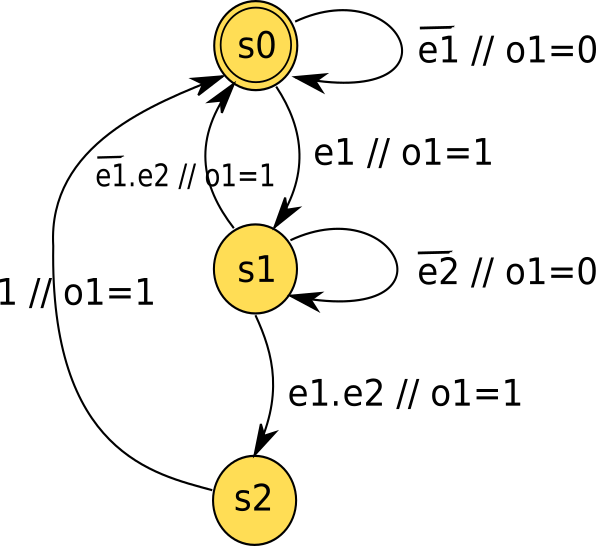
\includegraphics[scale=0.3]{./figures/ex-fsm-1.png}
\end{center}
\caption{FSM de l'exercice 1 et 2}
\label{fig2}
\end{figure}

C'est un automate de Mealy, car les sorties dépendent des transitions, et non pas seulement des états.

\subsection{Equations logiques de l'automate}
On cherche les équations logiques de la fonction "état suivant", ainsi que de la fonction de sortie de l'automate précédent. Ces deux ensembles
nous permettrons de réaliser concrètement le circuit. On suggère ici de procéder en 2 étapes.
La première consiste à conserver le nom {\it symbolique} des états tandis que la seconde fait apparaître l'{\it encodage} de ces états.
Dans la FSM à réaliser, en choisissant un encodage {\it one-hot}, trois bits seraient nécessaires pour encoder les états.
On va se limiter toutefois ici à un encodage {\it dense} où 2 bits seuls sont nécessaires. On s'appuie sur les tableaux génériques suivant \ref{tab1} et \ref{tab2},
qui permettent de procéder de manière systématique.
\begin{table}[htp]

  \centering
  \caption{Encodage symbolique (nom des états préservés)}\label{tab1}

  \begin{tabular}{|l|l|l|l||l|l|l|l|}
      \hline
      état courant & entrée 1 & ... & entrée n &  état suivant & sortie 1 & ... & sortie n \\ \hline
      ~        & ~    & ~         & ~            & ~            & ~        & ~   & ~        \\
      ~        & ~   & ~     & ~            & ~            & ~        & ~   & ~        \\
      \hline
  \end{tabular}

  \bigskip

  \caption{Encodage binaire (états encodés)}\label{tab2}

  \begin{tabular}{|l|l|l|l||l|l|l|l|l|l|}
    \hline
    Q1 & Q0 &  entrée 1 & ... & entrée n & D1 & D0 & sortie 1 & ... & sortie n \\ \hline
    ~        & ~  & ~  & ~  & ~  & ~  & ~  & ~        & ~   & ~        \\
    ~        & ~  & ~  & ~  & ~  & ~  & ~  & ~        & ~   & ~        \\
    \hline
  \end{tabular}

\end{table}

\boxed{Solution}

\begin{table}[h!]
    \begin{tabular}{|l|l|l||l|l|}
        \hline
        état courant & e1 & e2 & état suivant  & o1 \\ \hline
        S0           & 0  & X  & S0            & 0  \\
        S0           & 1  & X  & S1            & 1  \\
        S1           & X  & 0  & S1            & 0  \\
        S1           & 0  & 1  & S0            & 1  \\
        S1           & 1  & 1  & S2            & 1  \\
        S2           & X  & X  & S0            & 1  \\
        \hline
    \end{tabular}
\end{table}

Puis encodons les états symboliques S0,S1 et S2 par 00,01,10 :
\begin{table}[h!]
    \begin{tabular}{|l|l|l|l||l|l|l|}
        \hline
        Q1 & Q0 & e1 & e2 & D1 & D0 & o1 \\ \hline
        0  & 0  & 0  & X  & 0  & 0  & 0  \\
        0  & 0  & 1  & X  & 0  & 1  & 1  \\
        0  & 1  & X  & 0  & 0  & 1  & 0  \\
        0  & 1  & 0  & 1  & 0  & 0  & 1  \\
        0  & 1  & 1  & 1  & 1  & 0  & 1  \\
        1  & 0  & X  & X  & 0  & 0  & 1  \\
        \hline
    \end{tabular}
\end{table}
Attention : ne pas chercher les équations directement à partir de ce tableau ! Il manque des combinaisons !

\begin{table}[h]
\begin{tabular}{|l|l|l|l|l|}
\hline
        & /e1./e2 & /e1.e2 & e1.e2 & e1./e2 \\ \hline
/Q1./Q0 & 00      & 00     & 01    & 01     \\ \hline
/Q1.Q0  & 01      & 00     & 10    & 01     \\ \hline
Q1.Q0   & xx      & xx     & xx    & xx     \\ \hline
Q1./Q0  & 00      & 00     & 00    & 00     \\ \hline
\end{tabular}
\end{table}

A partir de ce dernier tableau, on peut déterminer les équations de D1,D0 et o1 :

%% $$D_1=\overline{Q_1}.Q_0.e_1.e_2$$
%% $$D_0=\overline{Q_1}.(\overline{Q_0}.e1+Q_0.\overline{e_2})$$
%% $$o_1=\overline{Q_1}.\overline{Q_0}.e_1+\overline{Q_1}.Q_0.e_2+Q_1.\overline{Q_0}$$


$$D_1=Q_0.e_1.e_2$$
$$D_0=\overline{Q_1}.\overline{Q_0}.e1+Q_0.\overline{e_2}$$
$$o_1=\overline{Q_1}.\overline{Q_0}.e_1+Q_0.e_2+Q_1$$

Puis le circuit numérique correspondant...


\section{Application}
Soit le diagramme états-transitions de la figure \ref{exo1}. On suppose que les entrées A et B proviennent de deux capteurs.
Les sorties sont S1,S2 et S3.

\begin{figure}[!h]
  \begin{center}
    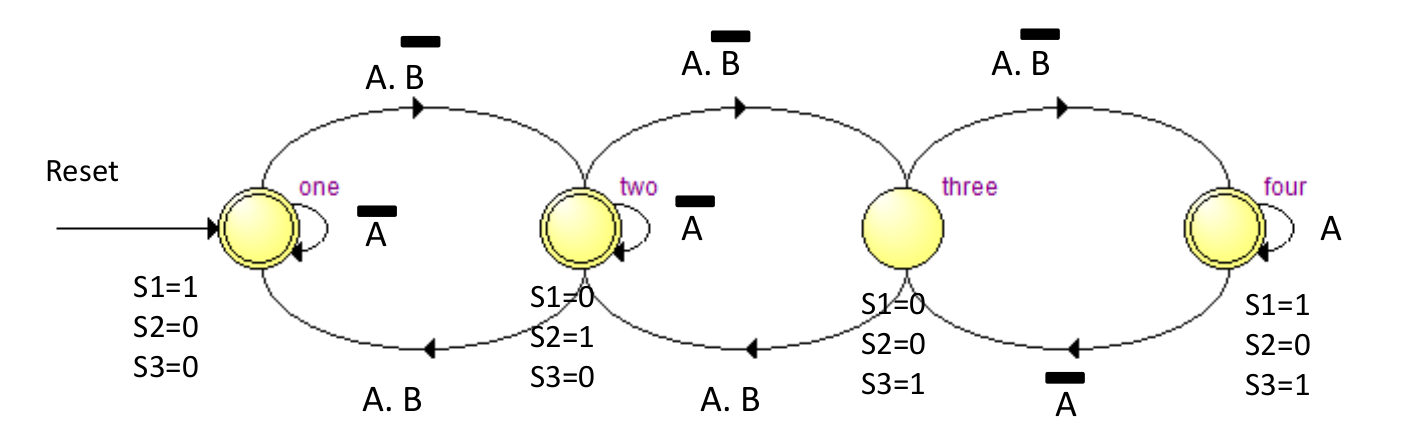
\includegraphics[scale=0.25]{./figures/exo1}
  \end{center}
  \caption{Diagramme états-transitions (à modifier).}
  \label{exo1}
\end{figure}

\begin{enumerate}
  \item Cette machine est-elle causale ? Si non, proposer une modification afin de la rendre causale.
  \item Proposer un encodage "one-hot" pour cette FSM, et un encodage dense.
  \item Etablir les équations de la fonction de transition. On rappelle que ces équations déterminent les entrées D des bascules d'état de l'automate.
  \item Etablir les équations de sortie.
  \item Dessiner la structure globale du circuit, en faisant apparaître, sous forme de nuage logique, les fonctions précédentes.
  \item Tenter de dessiner le circuit complet.
  \item Dessiner à part la connectique qui permet d'initaliser le système dans l'état
\end{enumerate}


\boxed{Solution}
C'est une solution proposée. Il en existe plusieurs.

\begin{enumerate}
  \item La machine n'est pas causale, car les conditions sont "incomplètes". On peut proposer de compléter ces conditions de manière totalement "ad hoc", pour que
  la FSM devienne causale. \textbf{Attention !} : ce "patch" sauvage est \textrm{dangereux} ! Cela signifie probablement que l'ingénieur qui a écrit la FSM initiale
  n'a pas une formulation robuste de son problème ! Dans un cas réel, le "patch" doit être soigneusement discuté afin de vérifier qu'il respecte le comportement attendu du système visé.

  \begin{figure}[!h]
    \begin{center}
      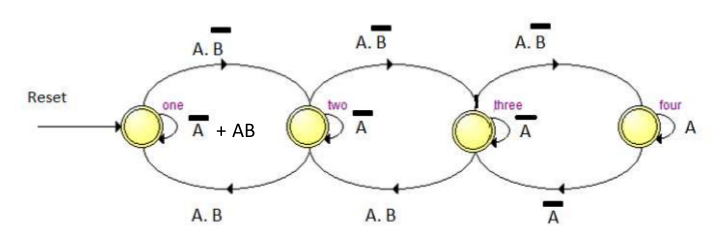
\includegraphics[scale=0.5]{./figures/correction_automate.png}
    \end{center}
    %\caption{Diagramme états-transitions (à modifier).}
    \label{solution}
  \end{figure}

  \item Encodage one-hot :
\begin{table}{htp}
  \caption{Encodage one-hot}
  \begin{tabular}{c|c}
    état  & code \\ \hline
    one   & 0001 \\
    two   & 0010 \\
    three & 0100 \\
    four  & 1000 \\
  \end{tabular}

  \caption{Encodage dense (exemple)}
  \begin{tabular}{c|c}
    état  & code \\ \hline
    one   & 00 \\
    two   & 01 \\
    three & 10 \\
    four  & 11 \\
  \end{tabular}

\end{table}

\item Appelons $Q_3$,$Q_2$,$Q_1$,$Q_0$ les (sorties des) bascules qui stockent chacun des bits d'états
dans le cas de l'encodage "one-hot". On conserve l'ordre indiqué dans les codes
précédents : on a ainsi $(Q_3,Q_2,Q_1,Q_0=(0,0,0,1)$ pour l'état "one".

On trouve les équations de transitions, à la simple lecture du diagramme, du fait de l'encodage one-hot :
$$
\begin{array}{lcl}
  D_0 & = & Q_0.(\overline{A}+A.B)+Q_1.A.B \\
  D_1 & = & Q_1.\overline{A}+Q_0.A.\overline{B}+Q_2.A.B\\
  D_2 & = & Q_2.\overline{A}+Q_1.A.\overline{B}+Q_3.\overline{A}\\
  D_3 & = & Q_3.A+Q_2.A.\overline{B}\\
\end{array}
$$

Les équations des sorties sont :
$$
\begin{array}{lcl}
  S_1 & = & Q_0+Q_3\\
  S_2 & = & Q_1\\
  S_3 & = & Q_2+Q_3\\
\end{array}
$$

\end{enumerate}

Le circuit ressemble à la figure \ref{circuit_template}.

\begin{figure}[!h]
  \begin{center}
    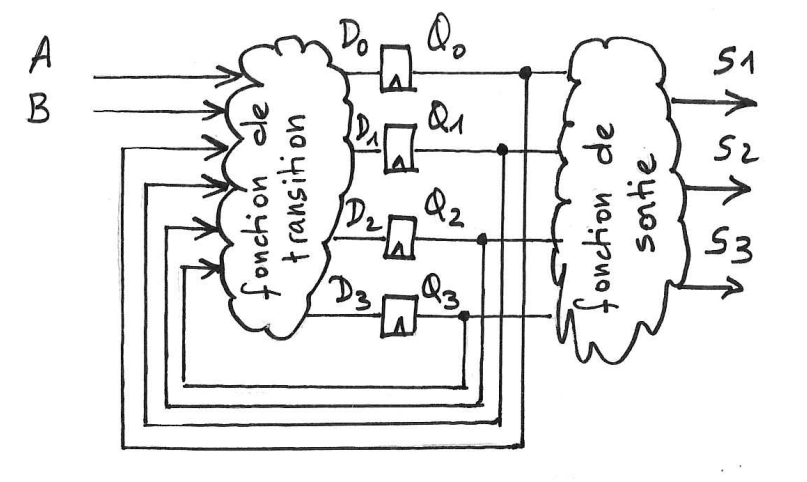
\includegraphics[scale=0.3]{./figures/circuit_template}
  \end{center}
  \caption{Schéma du circuit présentant les fonctions "état suivant" et "sortie" sous forme de nuage combinatoire.}
  \label{circuit_template}
\end{figure}

Le dessin à la main d'un tel circuit est très fastidieux...Il faut passer par des logiciels de synthèse automatique pour obtenir
un tel schéma.


%=================================================================================================================================
\section{Automate "détecteur de séquence"}

Il est fréquent de devoir détecter une séquence particulière dans un flux de données. Les automates se prêtent très bien à ce genre de détection. On peut citer :
\begin{itemize}
  \item L'analyse de paquets réseaux, détection de paquets interdits (entrants ou sortants) dont on connait une certaine signature numérique. C'est le travail de filtrage d'un "proxy", etc
  \item L'analyse de flux multimedia : par exemple "start codes" de séquences, dans un film (stocké en numérique, dans un format de compression).
  \item L'analyse génomique : il existe des accélérateurs FPGA dédiés à la reconnaisance de séquence du génôme, etc.
  \item etc.
\end{itemize}

\begin{figure}[!h]
  \begin{center}
    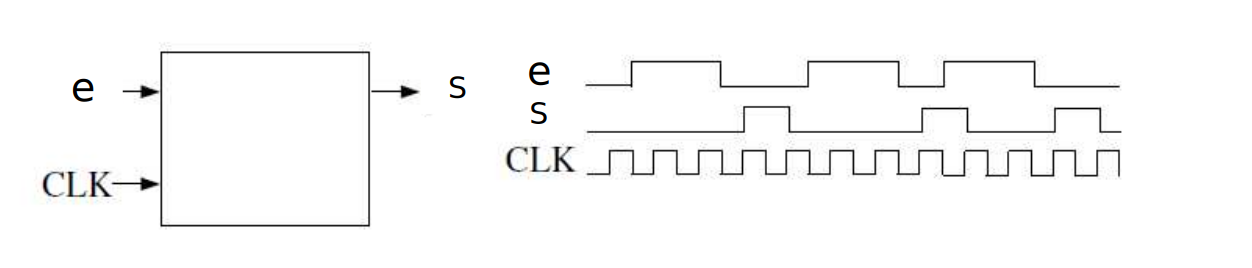
\includegraphics[scale=0.3]{./figures/exo2}
  \end{center}
  \caption{Schéma de principe du détecteur de séquence. Chronogramme associé.}
  \label{exo2}
\end{figure}

On considère le détecteur de séquence de la figure \ref{exo2}. Son rôle est de détecter les séquences "0-1-1-0" sur son unique entrée $x$.
Lorsque cette séquence est détectée, il émet un '1' sur sa sortie $y$. Un chronogramme est fourni à titre d'exemple. Notez que dans le flux
"0-1-1-0-1-1-0", la séquence apparaît deux fois !
\begin{enumerate}
  \item Proposer un diagramme états-transitions pour ce détecteur. On choisira une machine de Moore.
  \item Proposer un encodage dense des états.
  \item Réaliser le circuit.
\end{enumerate}


\boxed{Solution}

\begin{figure}[!h]
  \begin{center}
    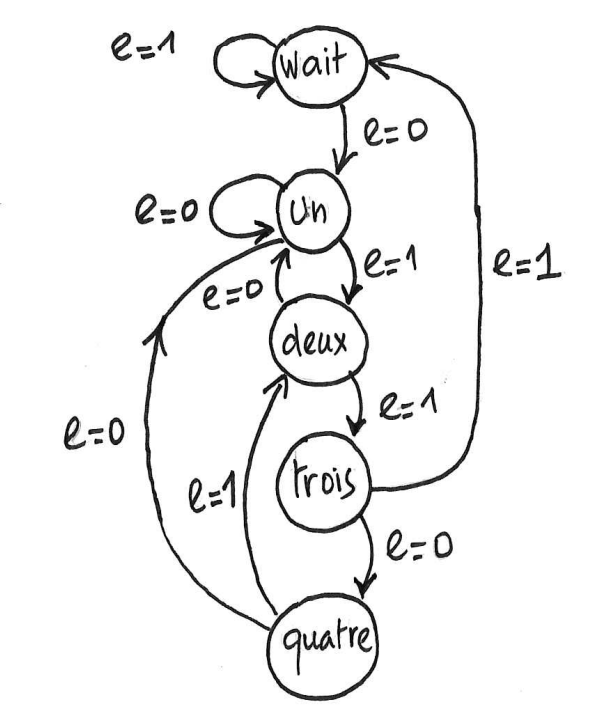
\includegraphics[scale=0.3]{./figures/fsm_detect}
  \end{center}
  \caption{Diagramme états-transitions pour le détecteur de séquences.}
  \label{fsm_detect}
\end{figure}

L'automate solution est décrit sur la figure \ref{fsm_detect}. On choisit l'encodage dense suivant :
\begin{table}[h!]
\begin{tabular}{c|c}
  état   & code \\ \hline
  wait   & 000 \\
  un     & 001 \\
  deux   & 010 \\
  trois  & 011 \\
  quatre & 100 \\
\end{tabular}
\end{table}

On a alors la table de séquencement suivante :\\

  \begin{tabular}{|l|l|l|l||l|l|l|l|l|l|l|}
    \hline
    $Q_2$ & $Q_1$ & $Q_0$ & e & $D_2$ & $D_1$ & $D_0$ & s \\ \hline
    0 & 0 & 0 & 0 & 0 & 0 & 1 & 0 \\ \hline
    0 & 0 & 0 & 1 & 0 & 0 & 0 & 0 \\ \hline
    0 & 0 & 1 & 0 & 0 & 0 & 1 & 0 \\ \hline
    0 & 0 & 1 & 1 & 0 & 1 & 0 & 0 \\ \hline
    0 & 1 & 0 & 0 & 0 & 0 & 1 & 0 \\ \hline
    0 & 1 & 0 & 1 & 0 & 1 & 1 & 0 \\ \hline
    0 & 1 & 1 & 0 & 1 & 0 & 0 & 1 \\ \hline
    0 & 1 & 1 & 1 & 0 & 0 & 0 & 0 \\ \hline
    1 & 0 & 0 & 0 & 0 & 0 & 1 & 0 \\ \hline
    1 & 0 & 0 & 1 & 0 & 1 & 0 & 0 \\ \hline
    \hline
  \end{tabular}\\

Cherchons maintenant les équations, en passant par des tableaux de Karnaugh.

% \begin{karnaugh-map}[4][4][1][$Q_2Q_1$][$Q_0E$]
%    \manualterms{1,1,1,1, 0,1,0,1, 0,0,1,0,0,1,1,1}
%    \implicant{13}{11}
%    \implicant{15}{10}
%    \implicantedge{0}{0}{8}{8}
%    \implicantedge{3}{3}{11}{11}
% \end{karnaugh-map}

\begin{karnaugh-map}[4][4][1][$Q_2Q_1$][$Q_0E$]
   \minterms{0,1,2,5,8}
   \maxterms{4,6,9,12,13}
   \terms{3,7,10,11,14,15}{X}
   \implicant{1}{7}
   \implicantcorner
\end{karnaugh-map}

On obtient la formule \boxed{D_0=Q_1.\overline{Q_0}+\overline{Q_1}.\overline{E}}

\begin{karnaugh-map}[4][4][1][$Q_2Q_1$][$Q_0E$]
   \minterms{5,6,8,12}
   \maxterms{0,1,2,4,9,12,13}
   \terms{3,7,10,11,14,15}{X}
   \implicant{5}{7}
   \implicant{7}{14}
   \implicantedge{12}{12}{14}{14}
\end{karnaugh-map}

On obtient la formule \boxed{D_1=Q_1.\overline{Q_0}.E+\overline{Q_1}.Q_0.E+Q_2.E}.

\begin{karnaugh-map}[4][4][1][$Q_2Q_1$][$Q_0E$]
   \minterms{9}
   \maxterms{0,1,2,4,5,6,8,12,13}
   \terms{3,7,10,11,14,15}{X}
   \implicant{9}{11}

\end{karnaugh-map}

On obtient la formule \boxed{D_2=Q_1.Q_0.\overline{E}}

\begin{karnaugh-map}[4][4][1][$Q_2Q_1$][$Q_0E$]
  \minterms{2,6}
  \maxterms{0,1,4,5,8,9,12,13}
  \terms{3,7,10,11,14,15}{X}
  \implicant{3}{10}
\end{karnaugh-map}

On obtient la formule \boxed{D_3=Q_2}

%=================================================================================================================================
\section{Automate "serrure numérique"}
L’accès à un local est protégé par une serrure codée associée à un
automatisme commandant la gâche électrique de la porte. La combinaison secrète est : A,D,C.

\begin{figure}[!h]
  \begin{center}
    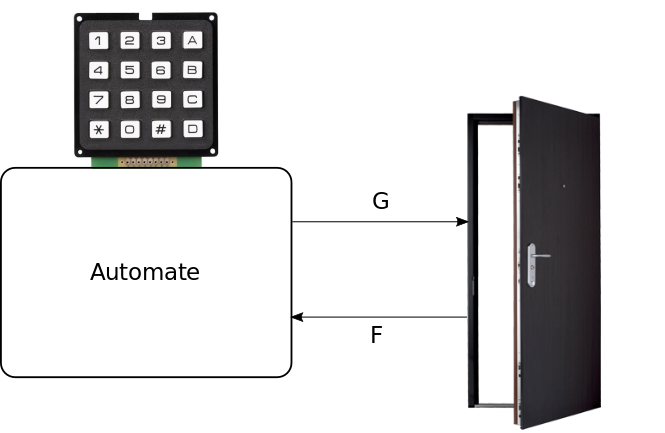
\includegraphics[scale=0.3]{./figures/porte.png}
  \end{center}
  \caption{Schéma de principe de la serrure numérique.}
  \label{exo2}
\end{figure}

Un capteur permet de connaître l'état de la porte : F indique son état. F vaut à 1 si la porte est Fermée à 0 si elle est ouverte.
G commande l’ouverture de la porte : si G=1 la porte peut être ouverte. Lorsque la porte se referme, on a G=0.
A l’ initialisation la porte est fermée, le contact de porte F=1.
On précise qu'on ne peut appuyer que sur un seul bouton à la fois.

\begin{enumerate}
  \item Proposer un automate de contrôle du dispostif.
  \item Discuter de la robustesse de la solution, et de son réalisme. Proposer des alternatives.
  \item Optionel : construire le circuit complet.
\end{enumerate}

\boxed{Solution}
Dans ce type de dispositifs, les {\it spécifications} du dispostif sont ambigües et sujettes
à interprétations. Cela est une constante dans ce type de dispostifs !
\begin{itemize}
  \item Par exemple, est-il réaliste de ne pas prendre en compte un temps limite d'attente entre deux actions d'appui sur
  un bouton ? On pourrait donc, dans un état donné, déclancher un {\it autre automate} dédié au décomptage du temps (timer).
  \item Ce timer est-il à déclancher {\it entre} deux appuis, ou dès qu'on commence la séquence ?
  \item De même, le sujet stipule que la porte "peut être ouverte" : cela ne signifie pas que le retrait de la gâche
  entraîne forcément l'ouverture de la porte : on devra donc là aussi attendre une action de l'utilisateur,
  probablement sur la poignée de la porte.
  \item S'il y a une poignée d'un côté de la porte, peut-on supposer qu'un {\it autre} utilisateur puisse
  ouvrir la porte, de manière inopinée pendant la tentative du premier utilisateur ? Etc...
\end{itemize}

Nous proposons ici une solution à peu près réaliste : dès que la lettre A est correctement entrée, un timer se déclanche.
Si la porte est par ailleurs ouverte (de l'intérieur), le dispositif se remet à l'état d'attente initial.

\begin{figure}[!h]
  \begin{center}
    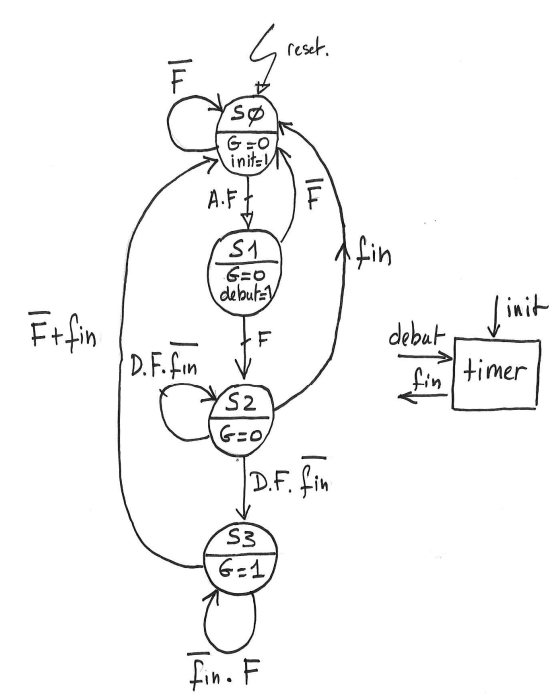
\includegraphics[scale=0.5]{./figures/my_solution.png}
  \end{center}
  \caption{Diagramme état-transition pour la serrure numérique. On fait appel à un autre dispositif numérique : un timer.}
  \label{my_solution}
\end{figure}

\end{document}
